\section{Mapping}

The setup studied in this project does not allow the translations of the EndoWrist. Although the models derived can be used on the full da Vinci robot, the mapping of the movements of the Geomagic Touch to the tool cannot be the same. As described in \secref{sec:geo_magic}, the GT can only actuates three joints, these joints are the one that needs to be used for the human to easily estimates the quality of the force feedback. It was decided to control the EndoWrist by controlling the roll, pitch and clamping independently. To do so, each of these three joints are assigned one vector. All three vectors are orthogonal to be able to sense the feedback of each joint individually.
The roll of the EndoWrist was associated to the roll of the GT. The clamp of the EndoWrist is associated to the radial vector going from the base of the GT to the end of the stylus. The pitch is controlled by the normal vector to the plan defined by the two previous vectors which is a vertical vector. The vectors in the horizontal plan are represented in \figref{fig:cartesian_polar}. The Cartesian z axis and the vector for the pitch of the EndoWrist are collinear and are not represented on the figure.
\\

\begin{figure}[H]
\centering
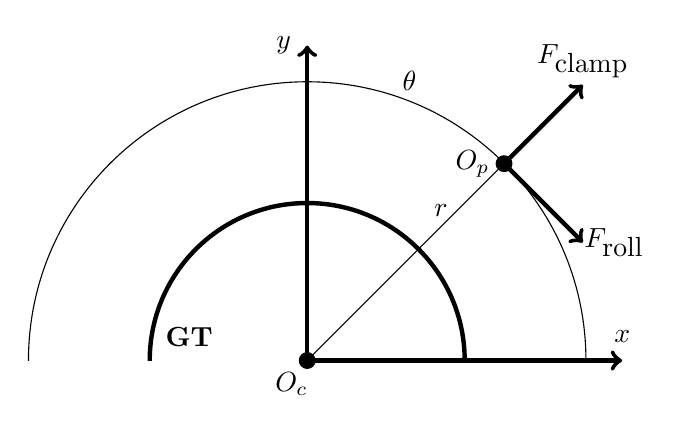
\begin{tikzpicture}
	% GT
	\begin{scope}
	    \clip (-2.1,0) rectangle (2.1,2.1);
	    \draw (0,0) circle(2)[ultra thick];
	\end{scope}
	\node at (-1.5,0.3) {$\textbf{GT}$};
	%Cartesian axis
	\draw [fill=black] (-0,-0) circle [radius=0.1];
	\draw [->,ultra thick] (0,0) -- (0,4);
	\draw [->,ultra thick] (0,0) -- (4,0);
	\node at (-0.3, 4) {$y$};
	\node at (4, 0.3) {$x$};
	\node at (-0.2, -0.3) {$O_c$};
	%end effector
	\draw [fill=black] (2.5,2.5) circle [radius=0.1];
	\begin{scope}
	    \clip (-3.55,0) rectangle (3.55,3.55);
	    \draw (0,0) circle(3.54);
	\end{scope}
	\draw (0,0) -- (2.5,2.5);
	\node at (2.1, 2.5) {$O_p$};
	%Cylindrical axis
	\draw [->,ultra thick] (2.5,2.5) -- (3.5,3.5);
	\draw [->,ultra thick] (2.5,2.5) -- (3.5,1.5);
	\node at (3.5,3.8) {$F_\textrm{clamp}$};
	\node at (3.9,1.5) {$F_\textrm{roll}$};
	\node at (1.3,3.55) {$\theta$};
	\node at (1.7,1.9) {$r$};

\end{tikzpicture}
\caption{Vectors in the Cartesian horizontal plan}
\label{fig:cartesian_polar}
\end{figure}

\begin{minipage}[t]{0.20\textwidth}
With:\\
\hspace*{8mm} $\theta$\\
\hspace*{8mm} $r$ \\
\hspace*{8mm} $O_c$ \\
\hspace*{8mm} $O_p$ 
\end{minipage}
\begin{minipage}[t]{0.68\textwidth}
\vspace*{2mm}
the angle between $\overrightarrow{y}$ and $\overrightarrow{O_c O_p}$\\ %$atan2(y,x)$, 
the distance $\overline{O_c O_p}$\\ %$\sqrt{x^2 + y^2}$, 
Origin of the Cartesian space\\
Position of the end-effector
\end{minipage}

The phantom\_omni node\cite{phantom_omni_github} used to communicate can only handle Cartesian positions and forces. Thus, conversion from cylindrical to Cartesian force vectors, see \eqref{eq:cylindrical_to_cartesian}, and from Cartesian coordinates to cylindrical coordinates, see \eqref{eq:cartesian_to_cylindrical}, are required.



\begin{equation} 
\begin{split}
	F_x &= F_\textrm{clamp}\cdot sin(\theta) + F_\textrm{roll}\cdot cos(\theta)\\
	F_y &= F_\textrm{clamp}\cdot cos(\theta) - F_\textrm{roll}\cdot sin(\theta)\\
	F_z &= F_\textrm{pitch}
\end{split}
%\caption{Conversion from cylindrical to Cartesian coordinates}
\label{eq:cylindrical_to_cartesian}
\end{equation}

\begin{minipage}[t]{0.20\textwidth}
With:\\
\hspace*{8mm} $(x,y,z)$ \\
\hspace*{8mm} $F_\textrm{clamp}$ \\
\hspace*{8mm} $F_\textrm{pitch}$ \\
\hspace*{8mm} $F_\textrm{roll}$ 
\end{minipage}
\begin{minipage}[t]{0.68\textwidth}
\vspace*{2mm}
the Cartesian coordinates of the GT\\
the force feedback from the clamp\\
the force feedback from the pitch\\
the force feedback from the roll
\end{minipage}

\begin{equation} 
\begin{split}
	&P_\textrm{roll} = a_\textrm{roll}\cdot \theta + b_\textrm{roll}\\
	&P_\textrm{pitch} = a_\textrm{pitch}\cdot z + b_\textrm{pitch}\\
	&P_\textrm{clamp1} = -a_\textrm{clamp} \cdot r + b_\textrm{clamp}\\
	&P_\textrm{clamp2} = a_\textrm{clamp} \cdot r - b_\textrm{clamp} 
\end{split}
%\caption{Conversion from Cartesian to cylindrical}
\label{eq:cartesian_to_cylindrical}
\end{equation}

\begin{minipage}[t]{0.20\textwidth}
With:\\
\hspace*{8mm} $P_i$\\
\hspace*{8mm} $a_i$ \\
\hspace*{8mm} $b_i$ 
\end{minipage}
\begin{minipage}[t]{0.68\textwidth}
\vspace*{2mm}
Position command sent to the joint $i$\\
constant scaling coefficient for joint $i$\\
constant scaling offset for joint $i$
\end{minipage}
